\documentclass[border=10pt]{standalone}
\usepackage{pgfplots}
\pgfplotsset{compat=1.18}
\begin{document}
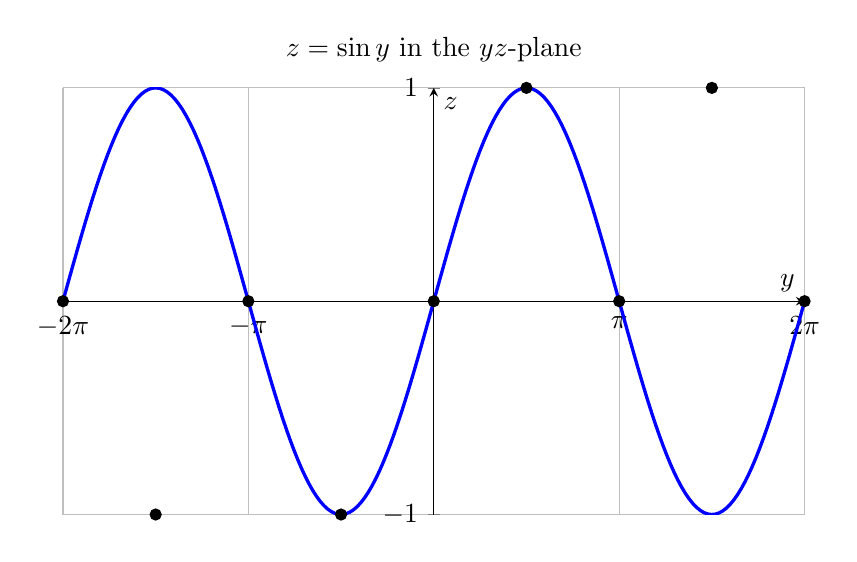
\begin{tikzpicture}
\begin{axis}[
  width=11cm, height=7cm,
  xlabel={$y$}, ylabel={$z$},
  title={$z=\sin y$ in the $yz$-plane},
  domain=-2*pi:2*pi,
  samples=200,
  ytick={-1,0,1},
  xtick={-6.283,-3.142,0,3.142,6.283},
  xticklabels={$-2\pi$,$-\pi$,$0$,$\pi$,$2\pi$},
  grid=major,
  axis lines=middle,
]
\addplot[blue, very thick] {sin(deg(x))};
\addplot[only marks, black, mark=*] coordinates {
  (-2*pi,0) (-3*pi/2,-1) (-pi,0) (-pi/2,-1)
  (0,0) (pi/2,1) (pi,0) (3*pi/2,1) (2*pi,0)
};
\end{axis}
\end{tikzpicture}
\end{document}